%
% poisson.tex
%
% (c) 2018 Prof Dr Andreas Müller, Hochschule Rapperswil
%
\documentclass[tikz]{standalone}
\usepackage{times}
\usepackage{txfonts}
\usepackage[utf8]{inputenc}
\usepackage{graphics}
\usepackage{ifthen}
\usepackage{color}
\usetikzlibrary{arrows,intersections}
\usetikzlibrary{math}
\begin{document}

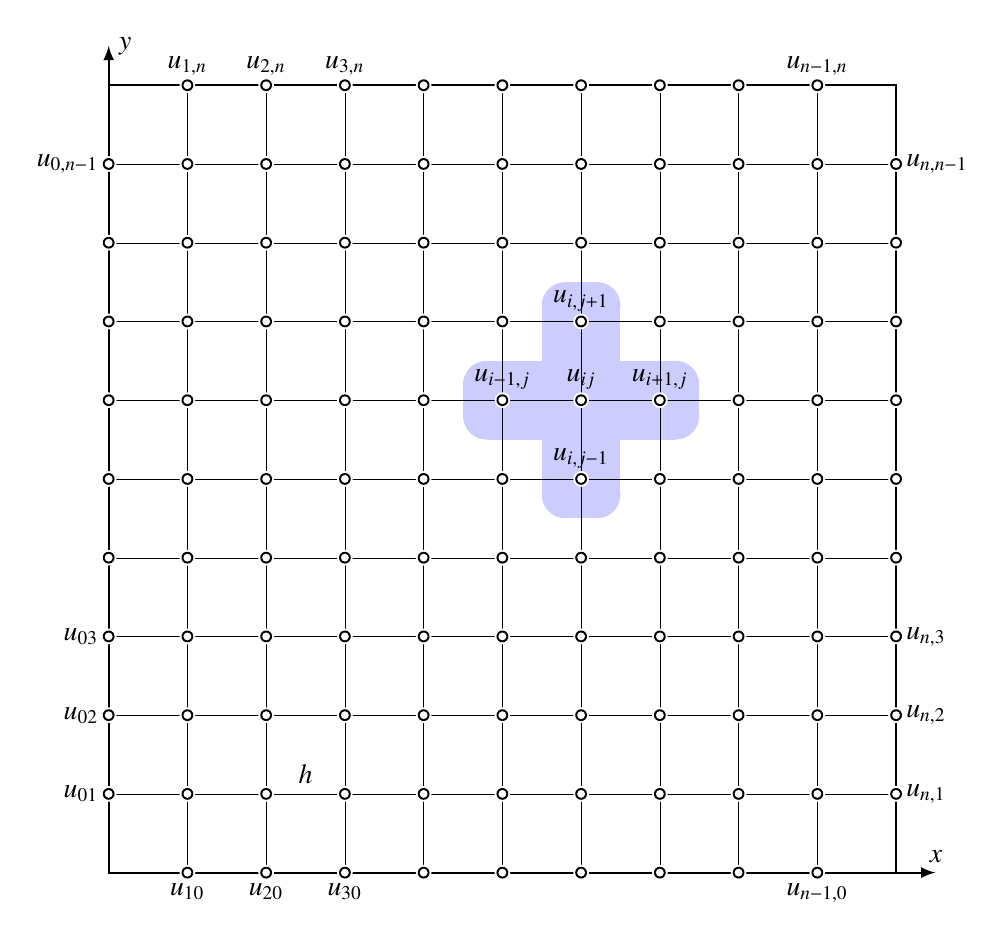
\begin{tikzpicture}[>=latex,thick]

\fill[color=blue!20] (5.8,7.2) circle[radius=0.3];
\fill[color=blue!20] (6.2,7.2) circle[radius=0.3];

\fill[color=blue!20] (5.8,4.8) circle[radius=0.3];
\fill[color=blue!20] (6.2,4.8) circle[radius=0.3];

\fill[color=blue!20] (4.8,5.8) circle[radius=0.3];
\fill[color=blue!20] (4.8,6.2) circle[radius=0.3];

\fill[color=blue!20] (7.2,5.8) circle[radius=0.3];
\fill[color=blue!20] (7.2,6.2) circle[radius=0.3];

\fill[color=blue!20] (4.8,5.5) rectangle (7.2,6.5);
\fill[color=blue!20] (5.5,4.8) rectangle (6.5,7.2);
\fill[color=blue!20] (4.5,5.8) rectangle (7.5,6.2);
\fill[color=blue!20] (5.8,4.5) rectangle (6.2,7.5);

\node at (2.5,1) [above] {$h$};
%\node at (1,3.5) [right] {$h_y$};

\foreach \x in {1,...,9}{
	\draw[line width=0.1pt] ({\x},0)--({\x},10);
}

\foreach \y in {1,...,9}{
	\draw[line width=0.1pt] (0,{\y})--(10,{\y});
}

\draw (0,0)--(0,10)--(10,10)--(10,0)--cycle;

\def\punkt#1#2{
	\fill[color=white] ({#1},{#2}) circle[radius=0.1];
	\fill ({#1},{#2}) circle[radius=0.075];
	\fill[color=white] ({#1},{#2}) circle[radius=0.05];
}

\foreach \x in {1,...,9}{
	\foreach \y in {1,...,9}{
		\punkt{\x}{\y}
	}
	\punkt{\x}{0}
	\punkt{\x}{10}
}

\foreach \y in {1,...,9}{
	\punkt{0}{\y}
	\punkt{10}{\y}
}

\node at (0,1) [left] {$u_{01}$};
\node at (0,2) [left] {$u_{02}$};
\node at (0,3) [left] {$u_{03}$};
%\node at (0,4) [left] {$u_{04}$};
%\node at (-0.1,7.1) [left] {$\vdots$};
\node at (0,9) [left] {$u_{0,n-1}$};

\node at (10,1) [right] {$u_{n,1}$};
\node at (10,2) [right] {$u_{n,2}$};
\node at (10,3) [right] {$u_{n,3}$};
%\node at (10,4) [right] {$u_{n,4}$};
%\node at (10.1,7.1) [right] {$\vdots$};
\node at (10,9) [right] {$u_{n,n-1}$};

\node at (1,0) [below] {$u_{10}$};
\node at (2,0) [below] {$u_{20}$};
\node at (3,0) [below] {$u_{30}$};
%\node at (4,0) [below] {$u_{40}$};
%\node at (7,0) [below] {$\mathstrut\dots$};
\node at (9,0) [below] {$u_{n-1,0}$};

\node at (1,10) [above] {$u_{1,n}$};
\node at (2,10) [above] {$u_{2,n}$};
\node at (3,10) [above] {$u_{3,n}$};
%\node at (4,10) [above] {$u_{4,n}$};
%\node at (7,10) [above] {$\mathstrut\dots$};
\node at (9,10) [above] {$u_{n-1,n}$};

\node at (6,6) [above] {$u_{ij}$};
\node at (6,7) [above] {$u_{i,j+1}$};
\node at (6,5) [above] {$u_{i,j-1}$};
\node at (5,6) [above] {$u_{i-1,j}$};
\node at (7,6) [above] {$u_{i+1,j}$};

\draw[->] (10,0)--(10.5,0) coordinate[label=$x$];
\draw[->] (0,10)--(0,10.5) coordinate[label={right:$y$}];

\end{tikzpicture}

\end{document}
